\newcommand{\tbontype}{\textsc{tbon}\textunderscore \textsc{tc}\textunderscore  \textsc{type}}
\newcommand{\tbonclasstype}{\textsc{tbon}\textunderscore \textsc{tc}\textunderscore \textsc{class}\textunderscore  \textsc{type}}
\newcommand{\tbonclustertype}{\textsc{tbon}\textunderscore \textsc{tc}\textunderscore \textsc{cluster}\textunderscore  \textsc{type}}
\newcommand{\tbonfeature}{\textsc{tbon}\textunderscore \textsc{tc}\textunderscore \textsc{feature}}
\newcommand{\tbongeneric}{\textsc{tbon}\textunderscore \textsc{tc}\textunderscore \textsc{generic}}

\section{Type Checker}
Test
\label{implementation-def-boolean-type}
\label{implementation-set-expressions}


\subsection{Building the Context}
\label{implementation-context-class-structure}
The type contexts for type checking of both informal and formal specifications are built using a hierarchy of types. This hierarchy is shown in figure \ref{fig:context-classes}.
\begin{figure}[H]
    \scalebox{0.6}{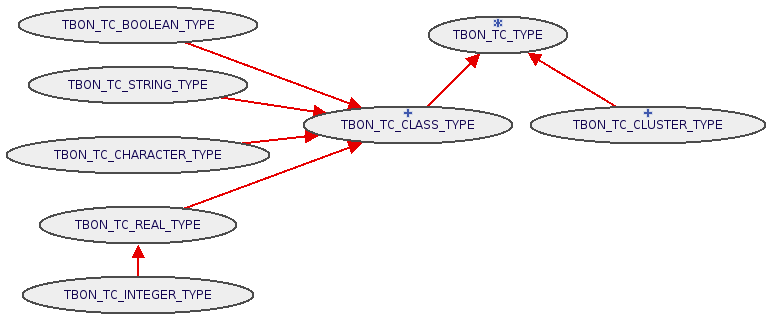
\includegraphics{images/context_classes3.png}}
    \caption[Context classes]{Hierarchy of classes used to build the type contexts}
    \label{fig:context-classes}
\end{figure}
A context, be it informal or formal, is built as a set of instances of \tbonclasstype   and \tbonclustertype   (declared as a set of \tbontype ). Due to the naming restrictions discussed in section \ref{design-type-names}, classes and clusters are kept in the same context for convenience and easy detection of name clashes. At any time, the instances in the context represent the defined types currently known at that point.
\paragraph{} Mapping from classes to features (in formal specifications) happens through association with a set of \tbonfeature . An instance of \tbonclasstype  is never associated with an undefined feature, but can be associated with an inconsistent or ill-typed feature (elaboration on this is found in section \ref{implementation-unresolved-elements}). Accordingly, the type of a feature is merely an association to an instance of \tbonclasstype .
\paragraph{} Analogous to the mapping from classes to features, mapping from classes to generics is done through association with a sequence of \tbongeneric  (generics cannot be stored in a set, as the order of the type parameters matters). A generic type has both a bounding and an actual class type. The association between these is explained in section \ref{implementation-generics}.

\subsection{Going Through the Phases}
\subsubsection{Unresolved Elements}
\label{implementation-unresolved-elements}

%Generics - explain association between bounding type and actual type.
\label{implementation-generics}
